

\subsection{Kinetics Action Recognition}
\label{section:experiments:kinetics}

\paragraph{Dataset.}
Kinetics-400~\cite{kinetics} is a widely used large-scale action recognition benchmark consisting of 240k training videos and 20k validation videos in 400 human action classes.
The performances are evaluated with the top-1 and top-5 accuracies. 
Note that about 10\% of the Kinetics-400 videos are not available on YouTube to be downloaded. It is not possible to reproduce the exact accuracies reported in the original paper; we train the action classifier over the available subset and treat this result as the baseline.

\paragraph{Training and evaluation.}
We follow the original training recipes of the baseline architectures in~\cite{feichtenhofer2019slowfast}.
We train models from scratch using the stochastic gradient descent optimizer for 250 epochs with batch size $64$ and initial learning rate $0.1$, which is decayed by cosine annealing. 
For a training video clip, $64$ consecutive frames are randomly sampled from a video and $T$ frames are sub-sampled with $\tau$ temporal stride as an input for video models. 
For every model, random resize crop and random horizontal flip are applied on training video clips as standard augmentations.
For evaluation, we use $3\times10$ view ensembles as in~\cite{feichtenhofer2019slowfast}, where $10$ clips are uniformly sampled along the temporal dimension from the entire video sequences and $3$ spatial regions are uniformly sampled along the longer side of the frames.


\paragraph{Network architecture.}
We use the SlowOnly, SlowFast~\cite{feichtenhofer2019slowfast}, and interaction preserved CSN (ip-CSN)~\cite{tran2019CSN} to show the impact of VideoMix on the video classification task. 
Every model is based on the ResNet architecture~\cite{resnet}. We denote the specific ResNet type with the suffix ``-(\#\ignorespaces depth)''.
We also denote each video model with frame length $T$ and temporal stride $\tau$ in the trailing bracket $(T\times\tau)$.
For example, SlowOnly-50 ($4\times16$) is based on the ResNet-50 architecture, considers $T=4$ input frames sub-sampled from the original $64$ frames with temporal stride $\tau=16$.
SlowFast-50 ($8\times8$) takes two separate input streams, the slow and fast pathways, each with $8$ and $32$ total number of input frames ($T$) with temporal strides ($\tau$) $8$ and $2$, respectively.


\paragraph{Kinetics-400 results.}


\begin{table}[t]
\small
\tabcolsep=0.08cm
\centering
\begin{tabular}{@{}lcccc@{}}
\toprule
{Model}                     & VideoMix & ~~top1~  & ~top5~~    & GFlops$\times$views \\ \midrule
I3D              &       &  72.1     &  90.3  &   108 $\times$ N/A        \\
Two-Stream I3D   &       &  75.7     &  92.0  &  216  $\times$ N/A      \\
Nonlocal-ResNet50   &       &   76.5     &  92.6  &  282 $\times$ 30         \\
\midrule
SlowOnly-50 ($4\times16$)   &      &    71.8  & 89.6  & 26 $\times$ 30 \\ 
SlowOnly-50 ($4\times16$)   & \checkmark     &    \textbf{72.7}  & \textbf{90.3} & 26 $\times$ 30  \\
\midrule
SlowOnly-50 ($8\times8$)    &      &    73.6  & 90.7  & 54 $\times$ 30 \\
SlowOnly-50 ($8\times8$)    & \checkmark     &    \textbf{74.9}  & \textbf{91.7} & 54 $\times$ 30 \\
\midrule
SlowFast-50 ($8\times8$)    &       &   75.9  & 91.9 & 65 $\times$ 30 \\
SlowFast-50 ($8\times8$)    & \checkmark     &    \textbf{76.6}  & \textbf{92.6} & 65 $\times$ 30 \\ \midrule
\end{tabular}
\caption{\textbf{Kinetics-400 action recognition results.} The inference cost is reported in the last column with GFlops of a single view $\times$ the number of views. 
N/A indicates the number of views are not available for us.}
\label{table:experiment:kinetics400}
\end{table}

We evaluate VideoMix on Kinetics-400 with SlowOnly and SlowFast networks~\cite{feichtenhofer2019slowfast} as the base network architectures.
SlowFast combines two branches: the slow branch for static spatial features and the fast branch for dynamic motion features.
SlowOnly only has the slow branch that is similar to the ResNet~\cite{resnet} architecture with 3D convolutional kernels.
The experimental results are shown in Table~\ref{table:experiment:kinetics400}.
The accuracies in the table are reproduced results\footnote{The original paper has reported the top-1 accuracies for {SlowOnly-50 ($4 \times 16$), SlowOnly-50 ($8 \times 8$), and SlowFast-50 ($8 \times 8$)} as $72.6$, $74.8$, and $77.0$, respectively. The difference is due to the 10\% unavailable videos in Kinetics-400 and smaller batch sizes due to GPU limitations.}.
We also report the inference cost (GFlops) of a single view (a temporal clip with spatial crop) as well as the number of views for the prediction of a single video.
We observe that VideoMix consistently improves the accuracy of baseline models. 
VideoMix achieves the top-1 accuracy of $72.7\%$, $74.9\%$, and $76.6\%$ for SlowOnly-50 ($4 \times 16$), SlowOnly-50 ($8 \times 8$), and SlowFast-50 ($8 \times 8$) with improvements of $+\mathbf{0.9}\%$, $+\mathbf{1.3}\%$, and $+\mathbf{0.7}\%$, respectively.
We also show that VideoMix-augmented SlowFast recognizer achieves a competitive performance ($76.6\%$) against other methods such as I3D~\cite{carreira2017quo} ($72.1\%$), Two-Stream I3D~\cite{carreira2017quo} ($75.7\%$), and Nonlocal-ResNet50~\cite{wang2018non} ($76.5\%$) which require more computational costs (GFlops) than the SlowFast architecture. 

\paragraph{Mini-Kinetics results.}

\begin{table}[t]
\centering
\begin{tabular}{@{}lcccc@{}}
\toprule
{Model}     & VideoMix        & top1  & top5 \\ 
\midrule
ip-CSN-50 ($8\times8$)     &                 &  74.8    &  91.9     \\
ip-CSN-50 ($8\times8$)     & \checkmark    & \textbf{75.9} & \textbf{93.1}    \\
\midrule
SlowOnly-50 ($4\times16$)     &             &   74.4    &   91.3    \\
SlowOnly-50 ($4\times16$)&  \checkmark               & \textbf{76.0} & \textbf{93.0}       \\
\midrule
SlowOnly-50 ($8\times8$)     &             &   77.5    &   93.2    \\
SlowOnly-50 ($8\times8$)     & \checkmark  & \textbf{79.2} & \textbf{94.1}       \\
\midrule
SlowFast-50 ($8\times8$)     &             &    79.5   & 93.9      \\
SlowFast-50 ($8\times8$)     & \checkmark  &    \textbf{81.9}  &  \textbf{95.1}      \\ 
\midrule
\end{tabular}
\caption{\textbf{Mini-Kinetics action recognition results.}
}
\label{table:experiment:mini-kinetics}
\end{table}


We also evaluate VideoMix on Mini-Kinetics as shown in Table~\ref{table:experiment:mini-kinetics}.
We observe that VideoMix improves the performance of various baseline architectures: ip-CSN-50~\cite{tran2019CSN}, SlowOnly-50 ($4\times16$), SlowOnly-50 ($8\times8$), and SlowOnly-50 ($8\times8$) with $\mathbf{75.9}\%$ ($\mathbf{+1.1}\%$), $\mathbf{76.0}\%$ ($\mathbf{+1.6}\%$), $\mathbf{79.2}\%$ ($\mathbf{+1.7}\%$) and $\mathbf{81.9}\%$ ($\mathbf{+2.4}\%$), respectively.








\paragraph{Ablation Studies.}

We conduct ablation studies on the Mini-Kinetics dataset.
SlowOnly-34 is used as the running baseline, where the BasicBlock is used as in ResNet-34~\cite{resnet}.
The results are shown in Table~\ref{table:experiment:albation}.

\section{Analysis}
In this section, we conduct ablation studies and a series of quantitative analyses to evaluate how various experimental designs and settings affect the outcomes of our distillation results.
\label{sec:5}
\subsection{Ablation Studies}
\label{sec:5-1}
In this subsection, we conduct an experiment named \textit{Direct Distillation}, where we train the retriever model directly using the relevance likelihood generated by LLM. More details of experiment setting can be found in Appendix \ref{sec:appendix-A}.
We compare the results of this approach with our proposed two-stage distillation scheme under the same LLM teacher model (i.e., GPT-4o), and the experimental results are shown in Table \ref{tab:tab03}.
The results indicate that the Direct Distillation method is less effective than our proposed Intermediate Distillation scheme, which further validates the rationality of the two-stage design of our proposed framework. 
% GPT-4o & 0.505 & 0.617 & 26.23 & 36.47 &  & 0.623 & 0.699 & 55.39 & 63.96 \\
% \vspace{-2mm}
\subsection{Impact of the Training Data Type} 
\label{sec:5-2}
\setlength{\tabcolsep}{1.5mm}{
\begin{table}[t]\label{tab:performance-drp}
    \centering
    \scalebox{1.0}{
    \resizebox{0.5\textwidth}{!}{
    \begin{tabular}{*{6}{c}}
      \toprule
      \multirow{3}*{\textbf{Method}} & \multirow{3}*{\textbf{Dataset}} & \multicolumn{3}{c}{\textbf{Evaluation Metrics}} & \\
      \cmidrule(lr){3-6}
      & & \textbf{EM$\uparrow$} & \textbf{F1$\uparrow$} & \textbf{HR@5$\uparrow$} \\
      \midrule
      Direct Distillation & NQ & 26.23 & 36.47 & 0.505 \\
      & TriviaQA & 55.39 & 63.96 & 0.623 \\
      \midrule
      Intermediate Distillation & NQ & 27.01 & 37.38 & 0.553 & \\
      & TriviaQA & 56.27 & 64.98 & 0.664 \\
      \bottomrule
    \end{tabular}
    }}
    \caption{Ablation studies on the effectiveness of two-stage distillation scheme design.}
    \label{tab:tab03}
    \vspace{-5mm}  % 调整与下文的间距
\end{table}}
\begin{figure}
    \centering
    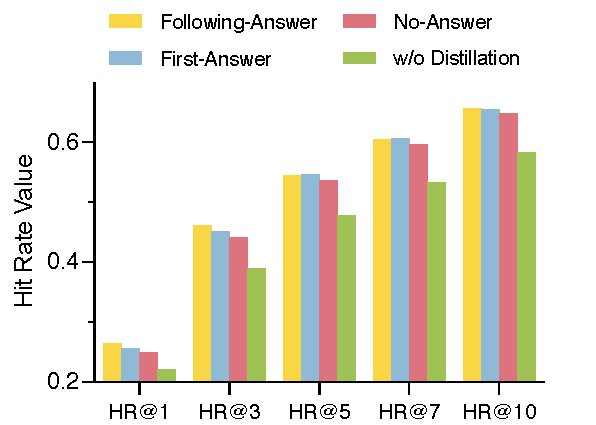
\includegraphics[width=0.45\textwidth]{latex/pic/fig4.pdf}
    \caption{The performance of retriever models across three types of training sets, which vary based on the initial appearance and placement of ground truth in the retrieved subsets.}
    \label{fig:04}
    \vspace{-10pt}
\end{figure}
Our previous experiment demonstrate that Rule-Based supervision signals, which places documents containing answers at the top, are ineffective and detrimentally impacting the retriever's performance.
This indicates that simply re-ranking documents based solely on the presence of ground truth (i.e., the correct answer) does not provide the high-quality text similarity insights required for effective distillation.
To delve deeper into the influence of the appearance and placement of ground truth in the re-ranking process, we categorize the initial retrieved document subsets $D_n$ based on \textit{NQ}'s queries into three categories:
(1) \textit{Following-Answer}: contains at least one document with the correct answer, but this kind of document is not at the first position in the subset. 
This data type is used in our experiments detailed in Section \ref{sec:4}.
(2) \textit{First-Answer}: contains at least one document with the correct answer, and this kind of documents is at the first position in the subset.
(3) \textit{No-Answer}: no documents in the subset contain the correct answer.

We follow the same training setting used in our primary experiments in Section \ref{sec:4}, and use GPT-4 Turbo as the LLM teacher model.
% The performance of the retriever models under these three data types of training are shown in Figure \ref{fig:04}.
% The results indicate that subsets with having ground-truth documents (i.e., Following-GT and First-GT) significantly improve retriever performance more than those without (i.e., No-GT).
% distilling the retriever model using subsets of relevant documents that contain the ground truth (i.e., Follow-GT and First-GT) produces better results compared to using the types that do not contain the answer (i.e., No-GT), and using Follow-GT proves to be more effective than using First-GT overall. 
Together with findings from the \textit{Rule-Based} experiments in Section \ref{sec:4}, the experiment results shown in Figure \ref{fig:04} indicate that considering the semantic similarity of the text is far more important than arranging documents containing the answers to the top for re-ranking in distillation training, as even the retriever under the \textit{No-Answer} data set training has notable improvements.

Moreover, as the \textit{Following-Answer} training data, where the correct answers are not ranked first initially, yields better training results than using the the \textit{First-Answer} training data, indicating that optimizing the ground truth placement in re-ranking also has a positive effect on the experimental results after the consideration of text similarity.
% Combined with the results from the Rule-Based experiments, this experimental results show that both prioritizing documents containing the answers and considering the semantic similarity of the text beyond just the answers determine the quality of the re-ranking distillation signals.

% This results suggests that re-ranking information containing the ground truth, especially those not initially ranked first, is a more effective distillation method. 
% Moreover, even the retriever under the No-GT data set training has notable improvements, showing that which highlights the advanced ranking capabilities of LLMs.
% \vspace{-1mm}
\subsection{Impact of the Training Set Size} 
\label{sec:5-3}
Our previous experiments demonstrate that our distillation framework significantly enhances retriever model performance with just 1,000 training instances. 
In this subsection, we explore how different training set sizes affect distillation effectiveness.
We use training sets of of 50, 100, 200, 500, 1000, and 2000 data instances from the \textit{Following-Answer} data type, with other settings consistent with our experiments in Section \ref{sec:4}. 
In addition, we use GPT-4 Turbo as our LLM teacher model.
% In addition to this, we use the same training setting as Section \ref{sec:5-1} uses to train the retriever model, and the experimental results are shown in Figure \ref{fig:05}.

Results in Figure \ref{fig:05} show that the performance of the retriever model improves significantly with training data with thousands of or even only hundreds of instances.
These empirical findings highlight the data efficiency of our proposed distillation scheme.
% initial increases in performance are significant with small training sets. 
In addition, although initial performance increases are notable with small training sets, the rate of improvement decreases as more training data is used.
This pattern indicates a \textit{scaling law} in distillation training, where further enhancements become increasingly difficult as the model's performance improves.
For models that already perform well, even marginal improvements require much more data, demanding greater training resources.
\begin{figure}
    \centering
    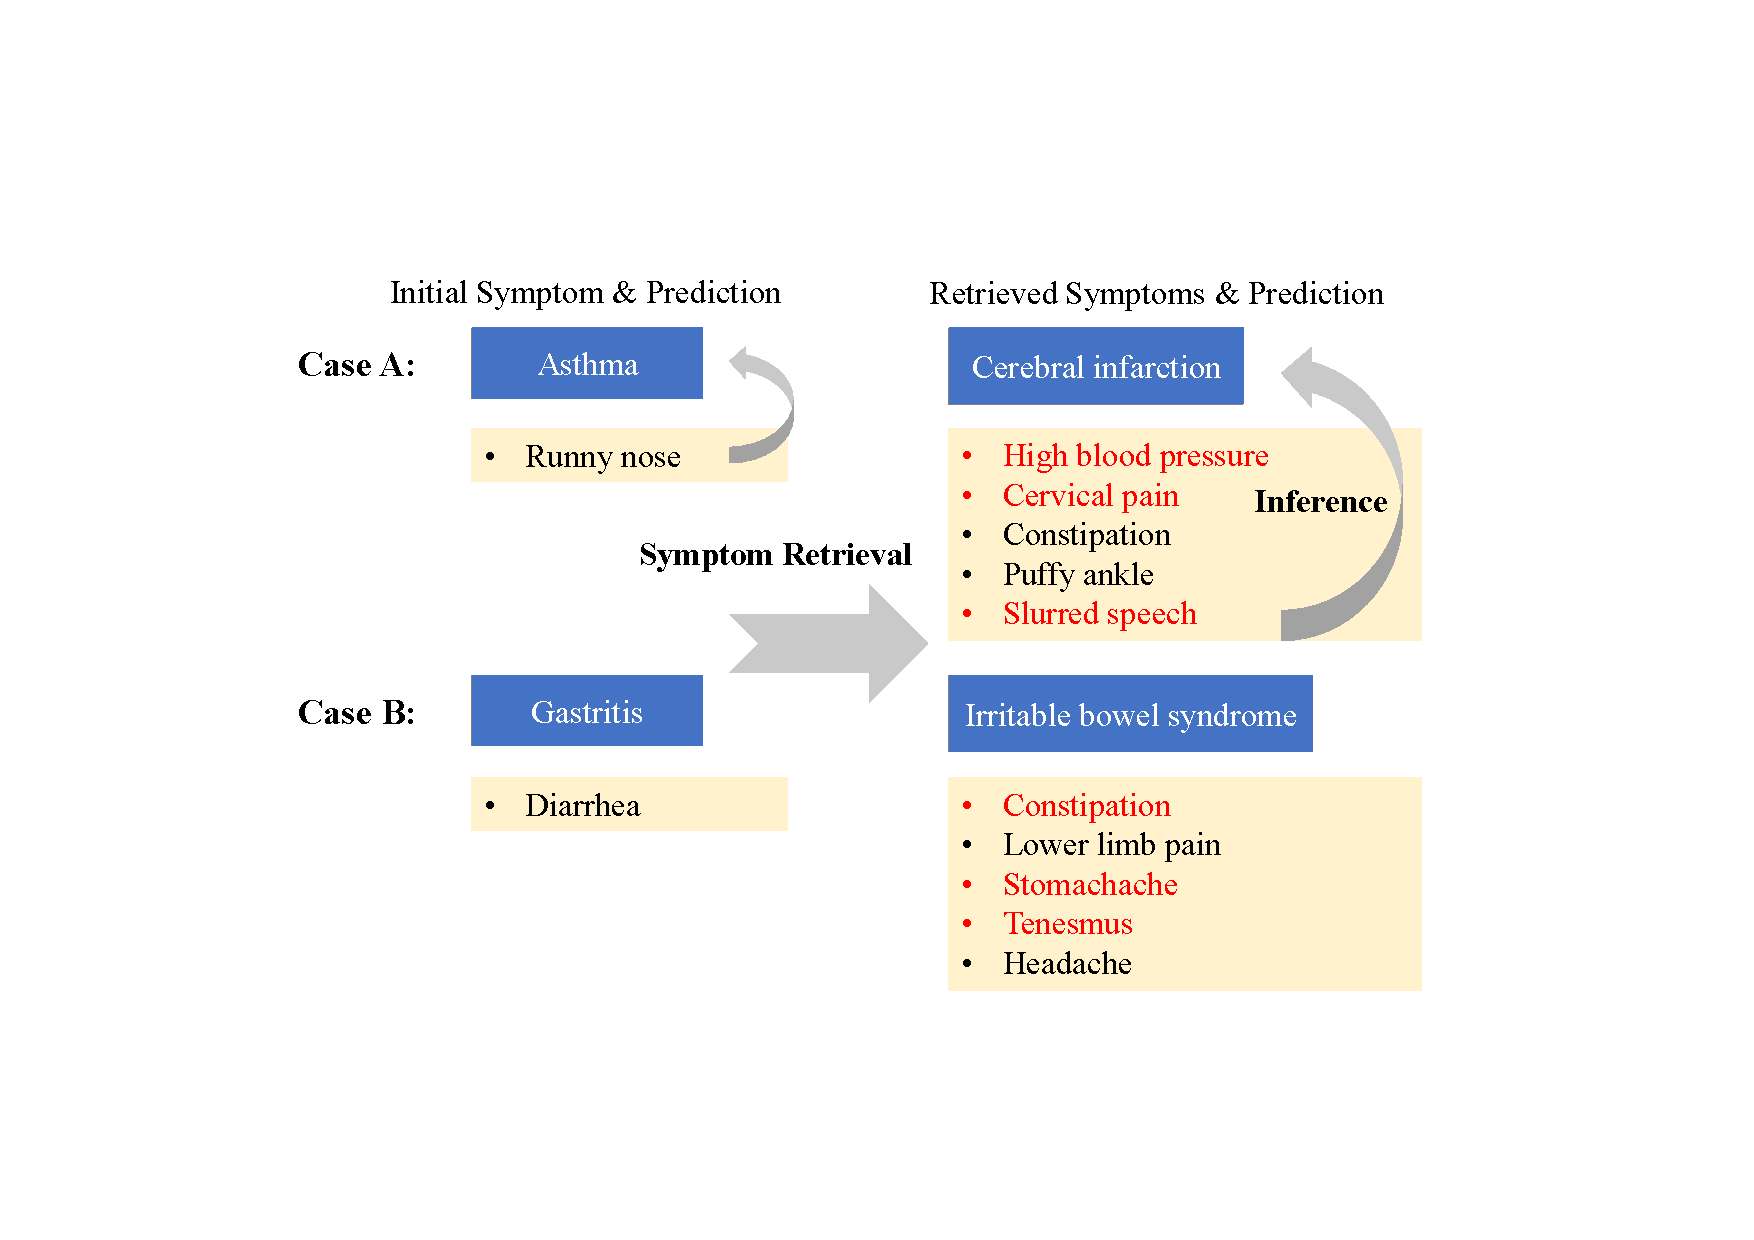
\includegraphics[width=0.5\textwidth]{latex/pic/fig5.pdf}
    \caption{The performance of retriever models under different training set size.}
    \label{fig:05}
    \vspace{-4mm}
\end{figure}

% For already high-performing retriever models, even small improvements require an exponentially larger amount of training data.
\subsection{Impact of the Re-ranking List Size}
\label{sec:5-4}
\begin{figure}[!htbp]
    \centering
    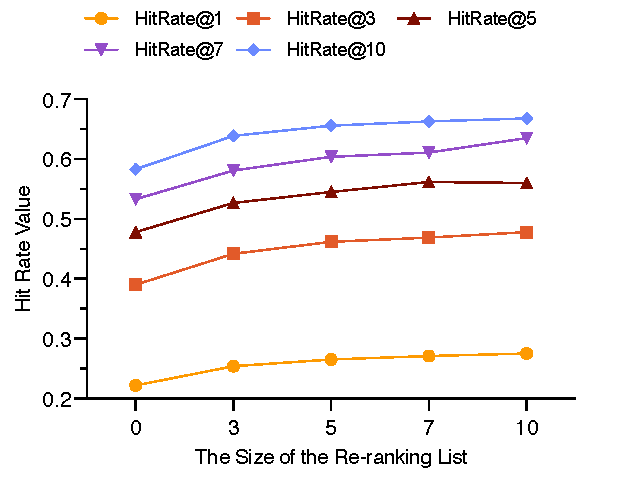
\includegraphics[width=0.5\textwidth]{latex/pic/fig6.pdf}
    \caption{The performance of retriever models under different size of the re-ranking list. The performance corresponding to 0 re-ranking list size represents the baseline retriever model performance.}
    \label{fig:06}
    \vspace{-4mm}
\end{figure}
In previous experiments, we set the re-ranking list to five documents (i.e., we retrieve five relevant documents each time).
Generally, larger re-ranking lists offer more supervision signals from LLMs, thus potentially enhancing the effectiveness of distillation training. 
To explore the impact of re-ranking list size on our distillation method, we vary the re-ranking list sizes, using the top-3, top-5, top-7, and top-10 documents from each relevant retrieved subset to conduct the distillation training.
% That is, during the initial data collection phase, the off-the-shelf retriever model returns the top-3, top-5, top-7, and top-10 relevant documents, respectively.
We keep other training settings consistent with those in our primary experiments in Section \ref{sec:4} and use GPT-4 Turbo as the LLM teacher model.

The experimental results shown in Figure \ref{fig:06} show that increasing the re-ranking list size progressively improves the effectiveness of the distillation training. 
As the list expands from re-ranking three documents to ten documents, the performance of the distilled retriever model consistently improves.
Moreover, compared with the retriever model's baseline performance, setting the size of the re-ranking list to 3 still significantly improves the retriever model's performance not only in HitRate@3 but also across broader metrics from HitRate@5 to HitRate@10.



% TODO in appendix:
% direct distill prompt cases
% case studies in metric v.s. LLM RAG performance


We first examine the impact of the mixture area hyperparameter $\alpha \in \{0.2,0.5,$ $1.0\text{(ours)},2.0\}$.
VideoMix at various $\alpha$ values exhibits stable performances, uniformly outperforming the vanilla baseline. VideoMix is not sensitive to the hyperparameter $\alpha$. 
When we reduce the chance of applying VideoMix on a minibatch to $prob$=$0.5$ (default is $prob$=$1.0$), the top-1 accuracy drops by $0.6$ percent point. The simple strategy of applying VideoMix on every video in the batch is a better choice.
When we increase the number of mixing videos (``\#videos") more than two, the performance significantly drops, which indicates that two videos are enough for VideoMix and mixing more than two videos may hinder the training convergence.

Temporal VideoMix and Spatio-temporal VideoMix are not as effective as the VideoMix (Spatial VideoMix), with only $+0.4\%$ and $+1.5\%$ boosts over the baseline.
Per-frame VideoMix independently applies VideoMix at every frame, ruining the temporal continuity of the VideoMix operation. It shows an even worse accuracy of 74.8\%, lower than the original model. Temporal continuity is an important ingredient for the video augmentation.

More ablation studies to see the effect of dataset sizes and applying other data augmentation methods together with VideoMix are provided in Appendix~\ref{appendix:more_baseline}.